\chapter{Extending FABRIK}

As we've established in earlier chapters, having a good algorithm for inverse kinematics can be a helpful tool for motion planning of robotic manipulators. It can be used in two ways:

\begin{itemize}
  \item Finding joint parameters that allow the manipulator to reach the target, and then looking for a way to reach the position with i.e. RRT.\ In this case, we don't mind if the IK algorithm is slow, since we are only computing it once. However, we want guarantees that a solution is found, if one exists.
  \item Finding a path with respect to the end effector with a different method, and using IK to find collision-free positions for the remaining joints. In this case, the priority is speed of computation, since it needs to be recomputed repeatedly.
\end{itemize}

For either case, the algorithm needs to be extended with a way to respect joint limits, and avoid collisions with surrounding obstacles.

\section{Adding joint limits to FABRIK}

When considering joint limits, computing the positions of points in space, as the original algorithm does~\ref{fig:fab}, is no longer sufficient; we need to consider what kind of joint we are currently dealing with, and what its orientation in space is.

Instead of points in space, we can use a complete kinematic model of our robot. This model, per DH convention, contains information about what joints and bodies the robot consists of, what parameters the joints are currently at, and calculates the corresponding matrices of each joint with respect to the rest of the world. Whenever a joint is moved, transformation matrices of the joints affected by this change are recomputed.

Since we want the kinematic model to stay connected, we can no longer easily disconnect the joint from the remainder of the configuration. Instead, a virtual copy of the manipulator is created and rooted at the target position.

[picture]

This way, the joints of the copy serve as points for the forward reaching stage, and the original joints serve as points for the backward reaching stage. Rather than detaching the current joint and moving it to the desired position, joints are moved at each step to minimize the distance, while respecting joint limits.

Finding the right joint parameters can be done by expressing the desired position in spherical coordinates~\cite{spherical}.

Spherical coordinates are an alternative way to describe points in space, different from the standard cartesian $x, y, z$ coordinates. In a spherical coordinate system, each point is uniquely described as $(r, \theta, \phi)$, where $r$ is the radial distance, which is any nonnegative number; $\theta$ is the azimuth angle, standardly ranging $0 \leq \theta < 2\pi$ and $\phi$ is the polar angle, standardly ranging $0 \leq \phi \leq \pi$. The limits are flexible, and we can change them to better match the possible joint rotations. For instance the polar angle can also range $-\pi \le \theta < \pi$, in which case the same points will be expressed slightly differently.

Using the inverse transformation matrix of our current joint, we can express the desired position in cartesian coordinates with respect to the joint. Then, the position can be converted to polar coordinates using the following equations:
\begin{equation}
  r = \sqrt{x^2 + y^2 + z^2}
\end{equation}
\begin{equation}
  \theta = \atantwo(\frac{x}{y})
\end{equation}

\begin{equation}
  \phi = \sin(\frac{z}{r})
\end{equation}

If the current joint allows for extension, we can extend or retract it to the correct radial distance. Rotations can be adjusted according to the two angles.

As the two stages alter iteratively, the two models converge to each other. Since the transformation matrices need to be recomputed repeatedly, the whole process is slower than the original algorithm, but gains several advantages.

\begin{itemize}
  \item The algorithm for forward and backward reaching is exactly the same, hence, it can be reused and the code is less sensitive to changes in the kinematic model.
  \item Both stages automatically respect the joint limits, since the model itself can validate the performed movements.
  \item Every movement of the original kinematic model can realistically be performed. We can ensure that our manipulator is always in a consistent state throughout the algorithm, which allows us to visualize the whole algorithm, generate intermediate steps for the purposes of animation, or stop the algorithm at any moment.
\end{itemize}

The most straightforward way to enforce that the joint limits are respected is to simply clamp the computed angles. If the algorithm computes an angle outside the range of the current joint,
the joint is instead set to the nearest feasible angle.

\begin{figure}[h]
    \centering
    \begin{minipage}{\textwidth}
        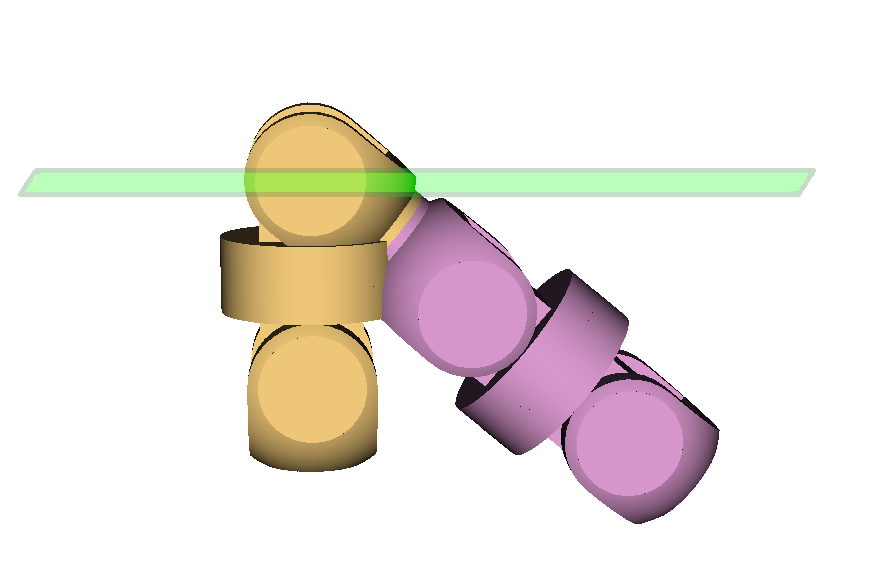
\includegraphics[width=.48\textwidth]{break_plane.png}
        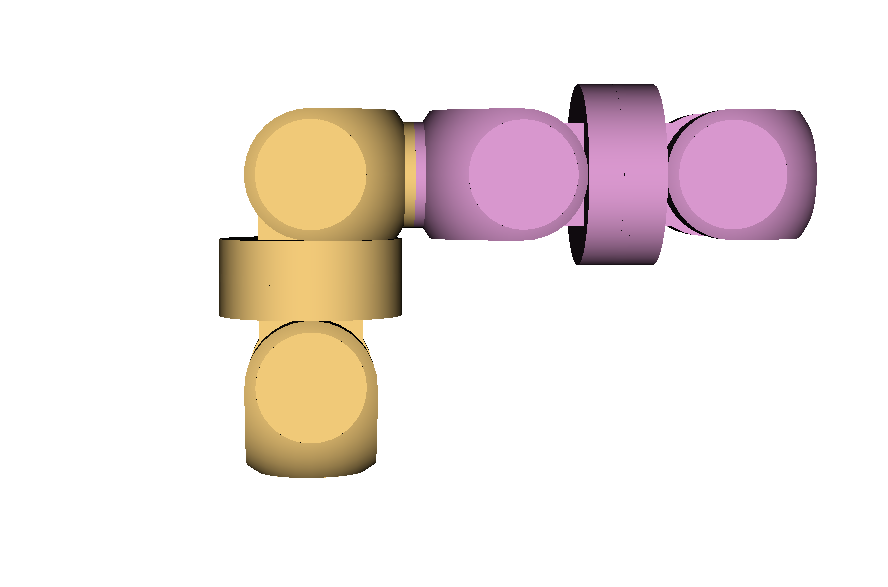
\includegraphics[width=.48\textwidth]{break_fixed.png}
    \end{minipage}
    \caption{The computed position violates the joint limit; the actual joint is clamped~\cite{Ondika2021thesis}.}\label{fig:break}
\end{figure}

While this limitation may prevent the algorithm from finishing in the current iteration, the other joints can make up for the limit and the manipulator is readjusted in the following iterations. In fact, as presented in~\cite{fabrik}, limitations on rotational joints can actually be helpful, in that more natural final poses are achieved.

The biggest problem we have to deal with comes when joints with only one degree of freedom are involved. Such joints can no longer rotate to an angle which minimizes the distance to the target joint, which means that we have to reason about the algorithm beyond the current joint for optimal results.

The optimal way to extend FABRIK to deal with this problem depends heavily on the build of the robot. Hence, in this part, the specifics of RoFI manipulators will be discussed; the core ideas may or may not translate to different manipulators.

Think back to the joints of the universal module~\ref{fig:um_rot}. When adapting the FABRIK algorithm to RoFI arms, we can treat each module as two joints. The joint between the two parts of a single module can only utilise the $\alpha$ or $\beta$ joint, hence, it is a simple rotational joint. As far as position of the next joint is concerned, the rotation of the $\gamma$ joint makes no difference. On the other hand, the joint between a universal module and the next component can utilise the $\gamma$ joint, and combine the two joints on the respective side to work as a ball joint and rotate in any direction. Passive modules or modules connected in a different direction can simply be viewed as a longer body between joints, and are not interesting for the algorithm.

The first idea that comes to mind may be to minimize the distance to the target joint position within the current limits. This is insufficient; if no special care is taken to account for joints that only have a single DoF, the manipulator will generally not reach the target.

The correct way to approach the problem is to align the one-dimensional joint in a way with the next target, so that only having one DoF is not limiting. Our implementation of FABRIK does exactly that: looking at the transformation created by the connection, the two DoF joint uses its mobility to place the next joint on the same plane as the target joint that follows it. As a result, the single DoF joint only needs to make a transformation in one plane, and the algorithm finds viable solutions to the constrained IK problem.

\begin{figure}[h]
    \centering
    \begin{minipage}{.6\textwidth}
        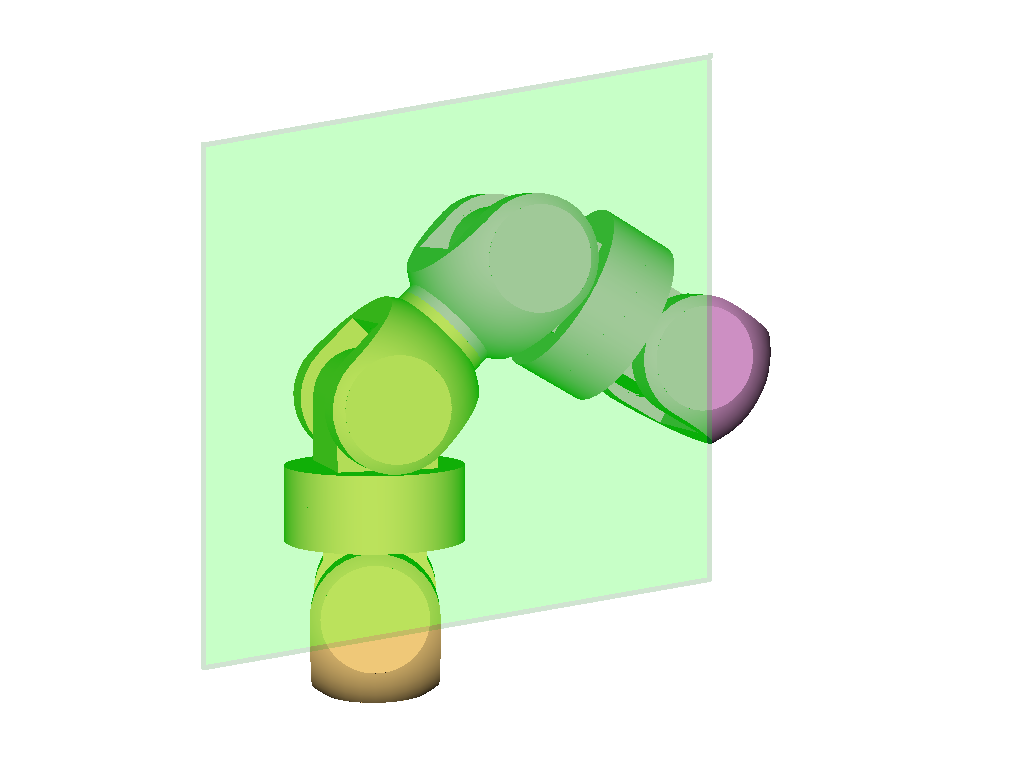
\includegraphics[width=\textwidth]{hinge_plane.png}
    \end{minipage}
    \caption{Visualization of the simplest connection of modules: the first module is rotated so that the first joint of the second module lies in the target plane of the next joint~\cite{Ondika2021thesis}}\label{fig:hinge}
\end{figure}

Depending on the way the modules are connected, there are several cases that need to be dealt with in the implementation. A short summary:

\begin{itemize}
  \item Joint between parts of the same module: perform rotation along the X axis with respect to the current target
  \item Joint with Z-Z connection: perform rotation along the X axis with respect to the current target, rotation along the Z axis with respect to the following target
  \item Joint with Z-X connection: perform rotation along the Z axis with respect to the current target
  \item Joint with X-Z connection: perform rotation along Z with respect to the position of the current joint, rotation along the X axis with respect to the following target
  \item Joint with X-X connection: perform rotation along the Z axis with respect to the current target
  \end{itemize}

Remeber that rotation along X is accomplished by the $\alpha$ and $\beta$ angles, while the rotation around Z corresponds to the $\gamma$ angle. The right angles are, as mentioned earlier, computed by fitting spherical coordinates to the possible movements of the joints; the azimuth angle (in radians) is clamped to $-\pi \le \theta < \pi$ to fit the $360\degree$ revolute Z joint, while the polar angle (in radians) is clamped to $-\frac{\pi}{2} \le \phi \le \frac{\pi}{2}$ to fit the $\left[-90\degree, 90\degree\right]$ X joint.

\section{Adding collision avoidance to FABRIK}
